% ==================== 公共物理模型与通信链路模型 ====================
% 说明：本章的公式是整个论文的“唯一口径”，问题一至问题四全部复用，
%       不允许在任何一问中另行定义（对应铁律 R4：物理口径唯一）。

山区场景下，地形起伏同时决定了无人机的爬升高度与通信链路的遮挡状态，而机队规模与电池周转又共同约束了任务的可行域。为使四个问题在同一物理口径下可比，本文先建立公共的航段几何、能耗、充电与链路模型，供四问共用。

\subsection{航段几何与作业高度}

\textbf{（1）巡航海拔。}航段的计划巡航海拔取该航段所经过的 DEM 像元的\textbf{最高地面高程}再加 50\,m 安全净空：
\begin{equation}
	\label{eq:1}
	H_{cruise}(i,j)=\max\{\mathrm{DEM}(p):p\in\overline{ij}\}+50\ \mathrm{m}
\end{equation}
其中 $\overline{ij}$ 表示节点 $i$ 到 $j$ 的水平直线段。这里必须强调是“沿线最高点”而非“两端点较高者”——如图~\ref{fig:legs}(c) 所示，S003 的航段沿线最高点为 503.6\,m，远高于其自身地面海拔 308.5\,m。

\textbf{（2）作业高度与爬升/下降高度。}调度中心 O01 的作业高度取其地面海拔，服务区 $S_i$ 取地面海拔 $+30$\,m。于是
\begin{equation}
	\label{eq:2}
	h^{+}(i,j)=H_{cruise}(i,j)-H_{op}(i),\qquad
	h^{-}(i,j)=H_{cruise}(i,j)-H_{op}(j)
\end{equation}
连续访问多个服务区时，每次投送后均从 30\,m 作业高度\textbf{重新爬升}，因此后续航段的 $h^{+}$ 需按该服务区的作业高度重新计算。

\textbf{（3）航段飞行时间。}按爬升、巡航、下降三段相加：
\begin{equation}
	\label{eq:3}
	\begin{aligned}
		t_{gij}={}&\frac{h^{+}_{ij}}{v_{g}^{\uparrow}}+\frac{d_{ij}}{v_{g}^{c}}\\
		        &+\frac{h^{-}_{ij}}{v_{g}^{\downarrow}}
	\end{aligned}
\end{equation}
其中 $d_{ij}$ 为投影平面上的水平直线距离。

\subsection{载荷—航程关系与最大安全载荷}

\textbf{（1）载荷—航程关系。}无人机的航程与能耗随载荷的变化是任务规划的基础，已有研究从推进功率角度给出了多种能耗模型\cite{dai2022uavenergy}。附件给出的标准航程随载荷的变化满足 $3/2$ 次幂关系：
\begin{equation}
	\label{eq:4}
	L_{g}(q)=L_{g0}-(L_{g0}-L_{gF})\cdot\left(\frac{q}{Q_{g}}\right)^{3/2},\qquad 0\le q\le Q_{g}
\end{equation}
该关系具有三条性质：$L_{g}(0)=L_{g0}$（空载标准航程）、$L_{g}(Q_{g})=L_{gF}$（满载标准航程）、且因指数 $3/2>1$，$L_{g}(q)$ 关于 $q$ \textbf{单调不增且下凸}。凸性意味着载荷的边际代价递增，这一性质将在第\ref{sec:q1}节解释“为何重载机型在远距离率先触底”。三种机型的曲线如图~\ref{fig:payload_range} 所示。

\begin{figure}[htbp]
	\centering
	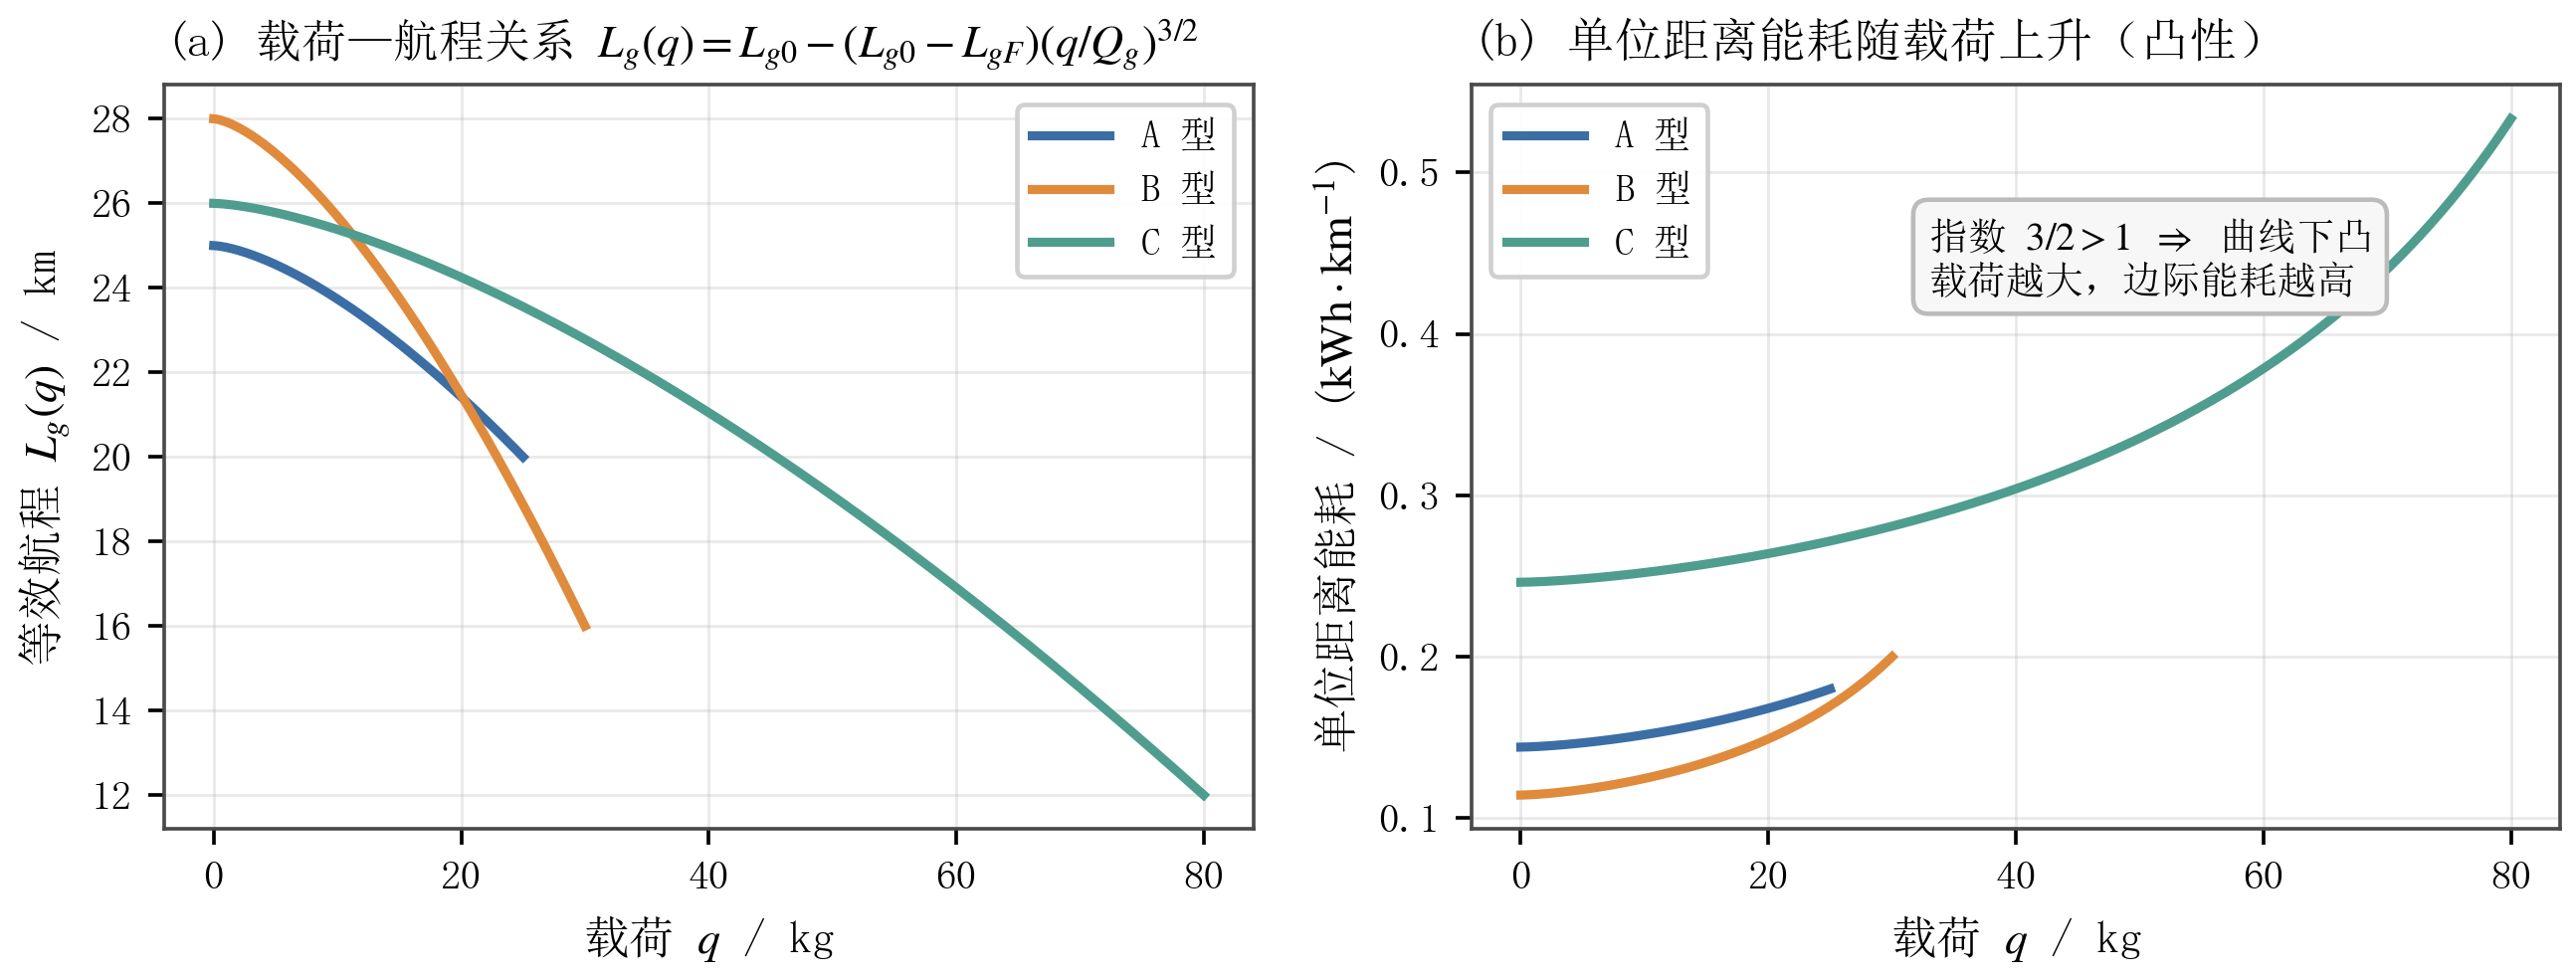
\includegraphics[width=0.98\textwidth]{figures/fig11_payload_range.png}
	\caption{载荷—航程关系与单位距离能耗}
	\label{fig:payload_range}
\end{figure}

由图~\ref{fig:payload_range}(a) 可见，A 型曲线最平缓（空载 25\,km、满载 20\,km），C 型最陡峭（26\,km 骤降至 12\,km）。图~\ref{fig:payload_range}(b) 把这一关系换算为单位距离能耗，可见载荷越大单位距离能耗越高，且增速越来越快——这正是凸性的物理含义。

\textbf{（2）航段能耗。}航段总能耗由水平巡航能耗与爬升附加能耗两部分构成：
\begin{equation}
	\label{eq:5}
	E_{gij}(q)=E_{gij}^{hor}(q)+E_{gij}^{up}(q)
\end{equation}
其中水平巡航能耗\textbf{由航程反推}（附件未给运输机巡航功率，由“飞满标准航程恰好耗尽可用能量”这一自洽口径确定）：
\begin{equation}
	\label{eq:6}
	E_{gij}^{hor}(q)=\frac{d_{ij}}{L_{g}(q)}\cdot E_{g}^{use}
\end{equation}
爬升附加能耗按势能除以爬升效率计算，其中质量取该航段上的实际总质量（含电池的空载质量加当前载荷）：
\begin{equation}
	\label{eq:7}
	E_{gij}^{up}=m\cdot g\cdot h^{+}_{ij}/\eta_{up},\qquad m=m_{g}^{empty}+q
\end{equation}
由于附件给出的下降能耗效率为 0，\textbf{下降段不单独计入能耗}，仅计入飞行时间。

\textbf{（3）最大安全载荷。}最大安全载荷由能量约束\textbf{取等号}定义：往返飞行（去程载货 $q$、回程空载）的总能耗恰好等于扣除了返航安全余量后的可用能量，
\begin{equation}
	\label{eq:8}
	E_{g}^{T}(q;d)=\sum_{(i,j)\in p}E_{gij}\big(q_{pij}\big)=(1-\rho_{g})\cdot E_{g}^{use}
\end{equation}
式中 $q_{pij}$ 为该航段上的实际剩余载荷。需要特别指出：由于 $L_{g}(q)$ 含 $3/2$ 次幂，$E_{g}^{T}$ 关于 $q$ 是\textbf{非线性}的，$(q/Q_{g})^{3/2}$ \textbf{没有初等反函数}，因此 $q_{max}$ 必须数值反解。本文利用 $E_{g}^{T}(q)$ 关于 $q$ 严格单调递增的性质，在 $[0,Q_{g}]$ 上用 \textbf{Brent 法}求根，并回代验证约束紧性，实测相对误差为 $5.6\times10^{-15}$。

最终的最大安全载荷还需与结构硬上限取小：
\begin{equation}
	\label{eq:9}
	q_{max}^{safe}=\min\big(q_{max}^{energy},\,Q_{g},\,\text{体积瓶颈对应质量}\big)
\end{equation}

\subsection{能源周转模型}

共享电池采用\textbf{两阶段等效充电模型}。设当前荷电状态为 $s\in[0,1]$，则充满所需时间为分段函数：
\begin{equation}
	\label{eq:10}
	t_{chg}(s)=T_{full}\cdot\left[0.65\cdot\frac{0.90-s}{0.90}+0.35\right],\qquad 0\le s<0.90
\end{equation}
\begin{equation}
	\label{eq:11}
	t_{chg}(s)=T_{full}\cdot0.35\cdot\frac{1-s}{0.10},\qquad 0.90\le s\le 1
\end{equation}
该模型有三个自检点：$t_{chg}(0)=T_{full}(0.65+0.35)=T_{full}$；在 $s=0.90$ 处上下两段均等于 $0.35T_{full}$，\textbf{函数连续}；$t_{chg}(1)=0$。其物理含义是充电前期（SOC $<90\%$）占满充时间的 65\%、后期（90\%$\sim$100\%）占 35\%，反映锂电池恒流—恒压两阶段特性。

电池的充电与换电策略对机队调度的影响已有专门研究\cite{kim2018batterycharging,mitici2022batteryswap}。资源占用规则为：同一资源的任务占用与充电时段\textbf{不得重叠}，不同资源可并行充电；同一机型的共享电池可在该机型的不同实体无人机间调度，\textbf{不同机型不可混用}。任务结束时的剩余 SOC 由可用能量与实际能耗算出，且不得低于返航电量下限 $\rho_{g}$。

\subsection{通信链路模型}

\textbf{（1）地形遮挡。}无人机的悬停高度与视距概率密切相关\cite{alhourani2014lap}。由链路两端的三维位置与 30\,m DEM 判断视线连线是否被地形遮挡，得到二值指示变量
\begin{equation}
	\label{eq:12}
	b_{ijt}=\begin{cases}0,&\text{视线无遮挡}\\1,&\text{视线被地形遮挡}\end{cases}
\end{equation}

\textbf{（2）接收门限与双向链路预算。}接收端的有效门限为灵敏度加衰落裕量，单向最大允许路径损耗由发射端与接收端参数共同决定：
\begin{equation}
	\label{eq:13}
	P_{th,b}=P_{sens,b}+M_{b}
\end{equation}
\begin{equation}
	\label{eq:14}
	L_{max,a\to b}=P_{t,a}+G_{t,a}+G_{r,b}-L_{sys}-P_{th,b}
\end{equation}
由于运输控制与状态回传都需要保障，\textbf{双向门限必须取两个方向中的较小值}：
\begin{equation}
	\label{eq:15}
	L_{max,a\leftrightarrow b}=\min\big(L_{max,a\to b},\,L_{max,b\to a}\big)
\end{equation}

\textbf{（3）传播损耗。}自由空间路径损耗为
\begin{equation}
	\label{eq:16}
	L_{FSPL,ijt}=32.45+20\log_{10}(f)+20\log_{10}(D_{ijt})
\end{equation}
这里存在一个\textbf{单位陷阱}：$f$ 的单位是 MHz，而 $D_{ijt}$ 的单位必须是 \textbf{km}。本文内部一律使用 SI 单位（距离以 m 存储），代入前必须除以 1000，否则将产生约 60\,dB 的系统性偏差。$D_{ijt}$ 为链路两端的\textbf{三维直线距离}（含高度差）。计入地形遮挡附加损耗后：
\begin{equation}
	\label{eq:17}
	\begin{aligned}
		L_{path,ijt}&=L_{FSPL,ijt}+L_{obs}\cdot b_{ijt},\\
		A_{ijt}&=1\iff L_{path,ijt}\le L_{max,i\leftrightarrow j}
	\end{aligned}
\end{equation}

\textbf{（4）通信三态判定。}综合上述判据，任一时刻的通信状态按优先级判定为三态：
\begin{equation}
	\label{eq:18}
	\text{状态}=\begin{cases}
		\text{直连}, & A(\text{运输机}\leftrightarrow G01)=1\\
		\text{中继}, & \text{直连不可用}\ \wedge\ A(\text{运输机}\leftrightarrow\text{中继})=1\\
		            & \qquad\wedge\ A(\text{中继}\leftrightarrow G01)=1\\
		\text{中断}, & \text{其余情况}
	\end{cases}
\end{equation}
即中继状态要求\textbf{接入段与回传段在同一时刻同时可用}，且不允许多跳转发、每架运输机在任一时刻只由 G01 或一架中继保障。

\subsection{统一计算器的耦合关系}

上述四组模型并非彼此独立：航段几何决定爬升高度，爬升高度同时进入能耗模型与视线遮挡判定；载荷通过 $L_{g}(q)$ 影响等效航程，进而影响能耗与最大安全载荷；能耗结果又反过来决定电池的剩余 SOC 与充电周转时间。图~\ref{fig:profile} 以最远的 O01\,$\to$\,S008 航段为例，展示了飞行剖面与能耗构成。

\begin{figure}[htbp]
	\centering
	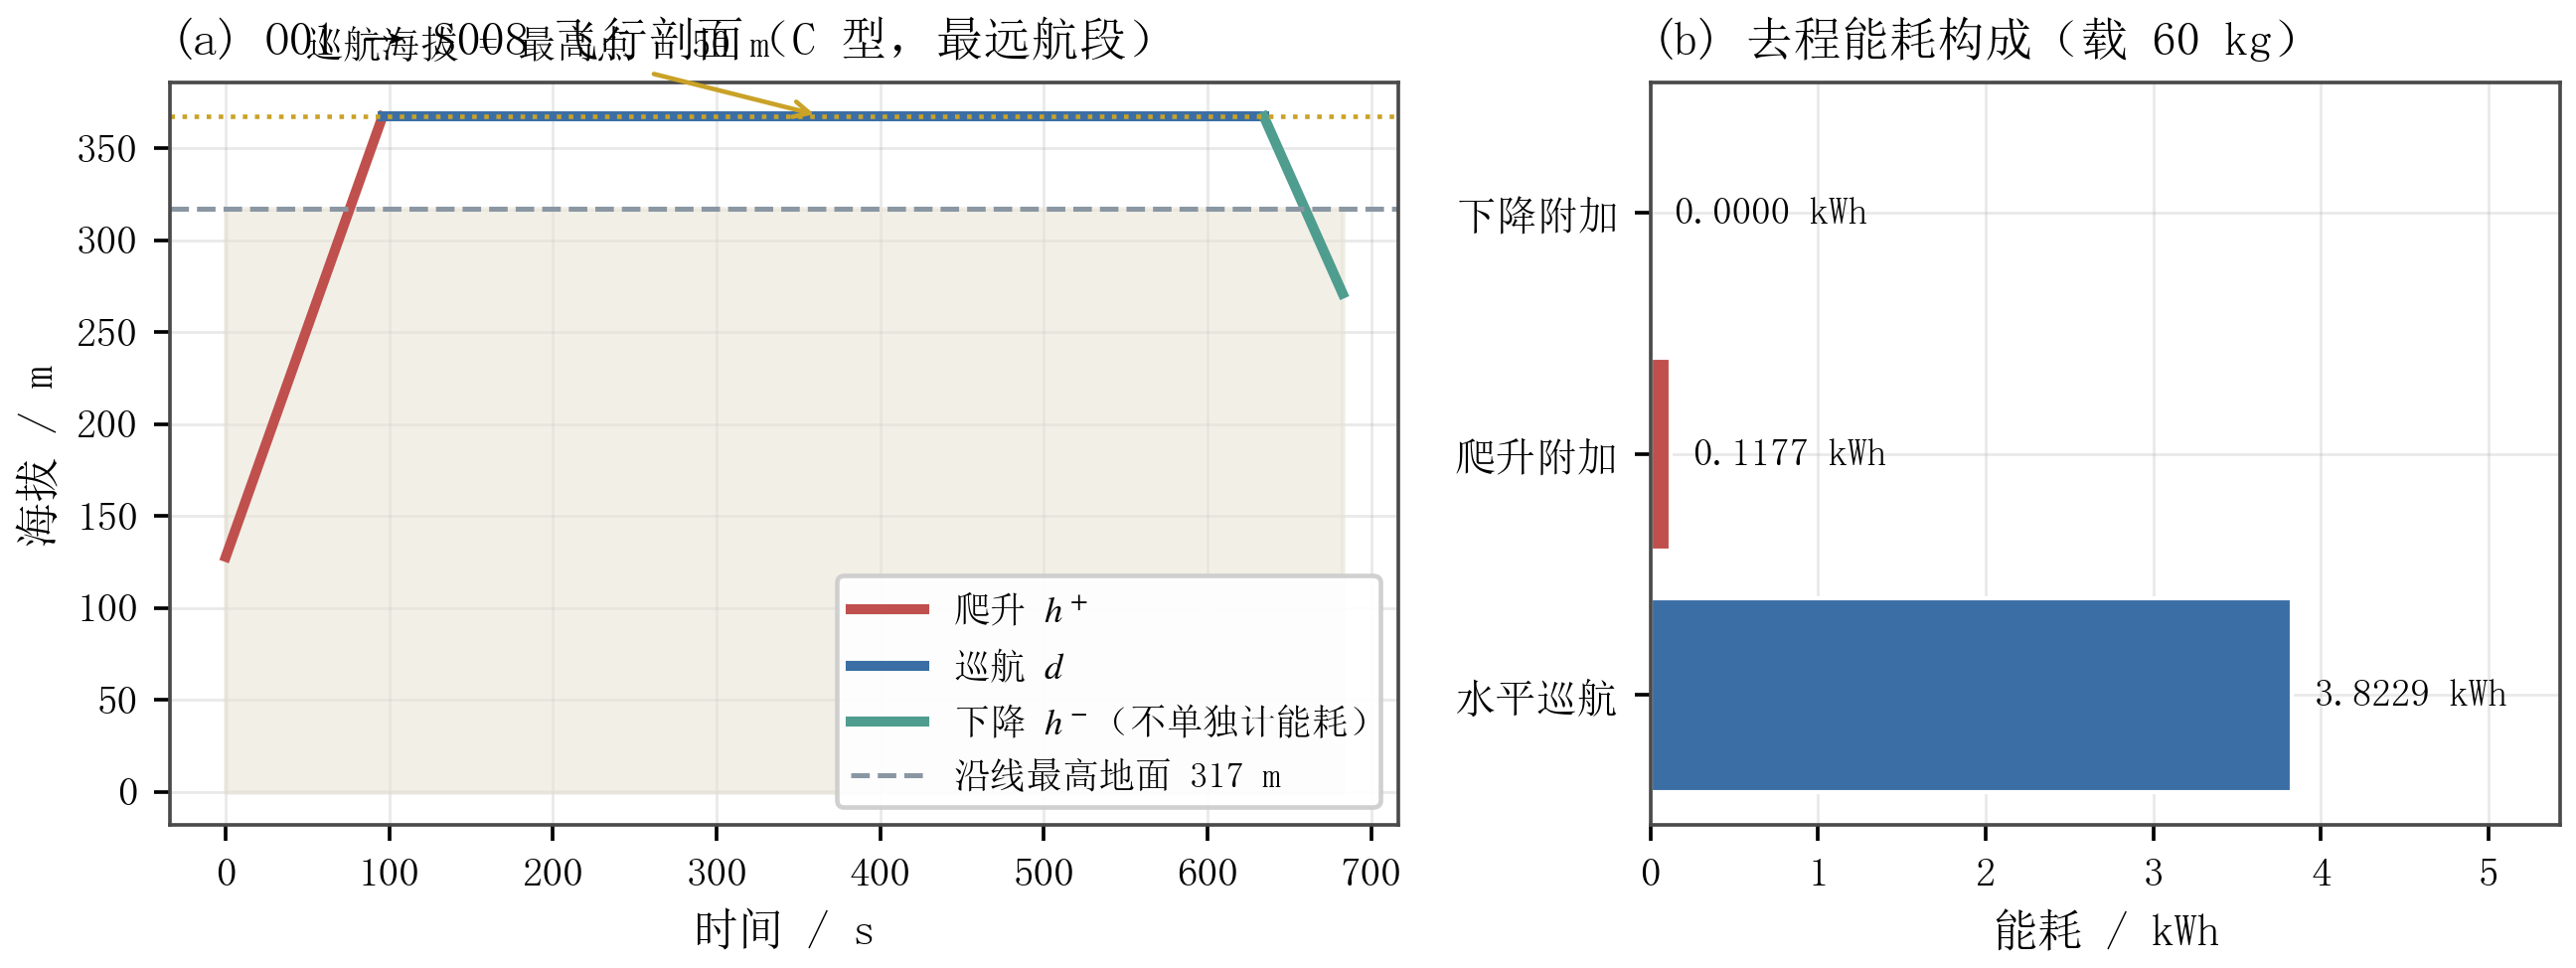
\includegraphics[width=0.98\textwidth]{figures/fig12_profile.png}
	\caption{飞行剖面与去程能耗构成}
	\label{fig:profile}
\end{figure}

由图~\ref{fig:profile}(a) 可见，无人机先爬升至“沿线最高点 $+50$\,m”的巡航海拔，平飞后下降至服务区作业高度；由于下降不单独计能耗，能耗只发生在爬升与巡航两段。图~\ref{fig:profile}(b) 表明在载重 60\,kg 时，水平巡航能耗显著大于爬升附加能耗——这解释了为何\textbf{航程（而非爬升）是决定架次能力的主要因素}，也说明“由航程反推巡航能耗”这一口径对结果的影响是主导性的。

至此，四问共用的公共模型建立完毕。问题一至问题四的全部计算均调用本模型，不再另行定义任何物理量，从而保证四问结果在统一口径下横向可比。
